
\documentclass{beamer}
\usepackage[latin1]{inputenc}
%\usetheme{Montpellier}
%\usetheme{Boadilla}
%\usecolortheme[RGB={204,51,255}]{structure}
%\usecolortheme[named=purple]{structure}
\usecolortheme[RGB={62,128,62}]{structure}
%\definecolor{dark}{rgb}{0.3,0.15,0.3}
%\definecolor{light}{rgb}{0.8,0.6,0.8}
%\definecolor{reddish}{rgb}{.5,0.15,0.15}
\definecolor{dark}{rgb}{0.5,0.3,0.4}
%\definecolor{light}{rgb}{0.8,0.6,0.8}
\definecolor{reddish}{rgb}{.7,0.25,0.25}
\definecolor{greenish}{rgb}{.25,0.7,0.25}
\definecolor{blueish}{rgb}{.25,0.25,0.7}
\definecolor{purple}{rgb}{.5,0.0,0.5}
\usepackage{graphicx}
\usepackage{pstricks}

\setbeamertemplate{navigation symbols}{}

\newcommand{\crish}{\color{reddish}}
\newcommand{\cbla}{\color{black}}
\newcommand{\cred}{\color{red}}
\newcommand{\cblu}{\color{blue}}
\newcommand{\cgre}{\color{green}}

\newcommand{\sm}{\color{reddish}$}
\newcommand{\fm}{$\color{black}{}}

\newcommand{\letter}[1]{\color{blue}\texttt{#1}\color{black}}
\newcommand{\binary}[1]{\color{red}\texttt{#1}\color{black}}

\usepackage{tikz}
\usetikzlibrary{arrows,decorations.markings,positioning}
\usepackage{epstopdf}
\usetikzlibrary{fit}

\title[Information Theory lecture 4]{Mutual information: lecture 4}
\author{COMSM0075 Information Processing and Brain}
\institute{\texttt{comsm0075.github.io}}
\date{September 2020}

\begin{document}

\maketitle

\begin{frame}{The chain rule for entropy}

\crish
$$
H(X,Y)=H(X)+H(Y|X)
$$ \cbla 

\end{frame}

\begin{frame}{$H(X,Y)=H(X)+H(Y|X)$}
\begin{center}
  
  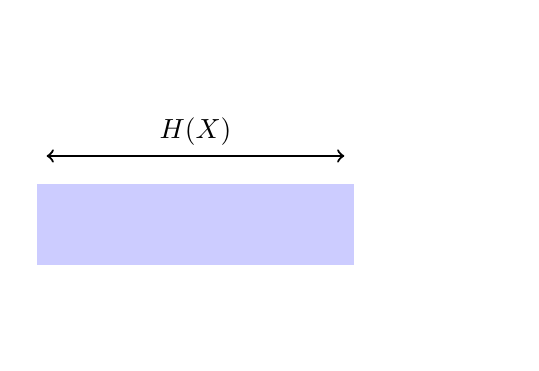
\begin{tikzpicture}
    \draw[help lines,draw=black!0] (0,0) grid (6,4);
    \node[fit={(0,1) (4,2)}, inner sep=0pt, draw=blue!20, fill=blue!20,thick] (X) {};
    \node[above = 0.75cm of X.east](Xleft){};
    \node[above = 0.75cm of X.west](Xright){};
    \draw[<->, thick, draw=black] (Xleft) -- (Xright) node[above,midway](HX){$H(X)$};
  \end{tikzpicture}

  \end{center}
  
 \end{frame}


\begin{frame}{$H(X,Y)=H(X)+H(Y|X)$}
\begin{center}
  
  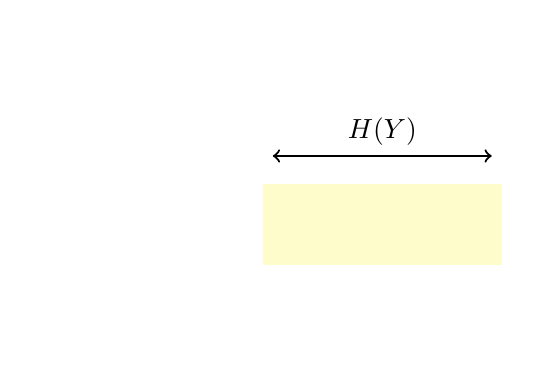
\begin{tikzpicture}
    \draw[help lines,draw=black!0] (0,0) grid (6,4);
    \node[fit={(3,1) (6,2)}, inner sep=0pt, draw=yellow!20, fill=yellow!20,thick] (Y) {};
    \node[above = 0.75cm of Y.east](Yleft){};
    \node[above = 0.75cm of Y.west](Yright){};
    \draw[<->, thick, draw=black] (Yleft) -- (Yright) node[above,midway](HY){$H(Y)$};
  \end{tikzpicture}

  \end{center}
  
 \end{frame}


\begin{frame}{$H(X,Y)=H(X)+H(Y|X)$}
\begin{center}
  
  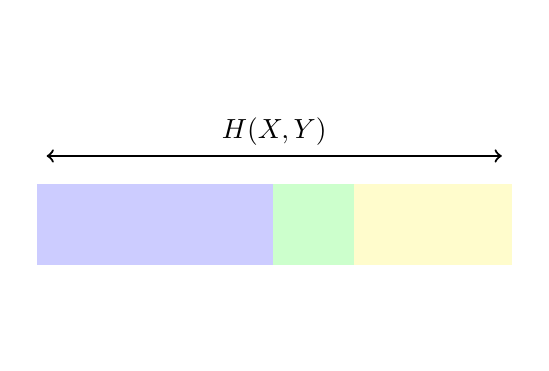
\begin{tikzpicture}
    \draw[help lines,draw=black!0] (0,0) grid (6,4);
    \node[fit={(4,1) (6,2)}, inner sep=0pt, draw=yellow!20, fill=yellow!20,thick] (X) {};
    \node[fit={(0,1) (3,2)}, inner sep=0pt, draw=blue!20, fill=blue!20,thick] (Y) {};
    \node[fit={(3,1) (4,2)}, inner sep=0pt, draw=green!20, fill=green!20,thick] (XcapY) {};
    \node[above = 0.75cm of X.east](Xleft){};
    \node[above = 0.75cm of X.west](Xright){};
    \node[above = 0.75cm of Y.east](Yleft){};
    \node[above = 0.75cm of Y.west](Yright){};
    \draw[<->, thick, draw=black] (Xleft) -- (Yright) node[above,midway](HXY){$H(X,Y)$};
  \end{tikzpicture}

  \end{center}
  
 \end{frame}


\begin{frame}{$H(X,Y)=H(X)+H(Y|X)$}
\begin{center}
  
  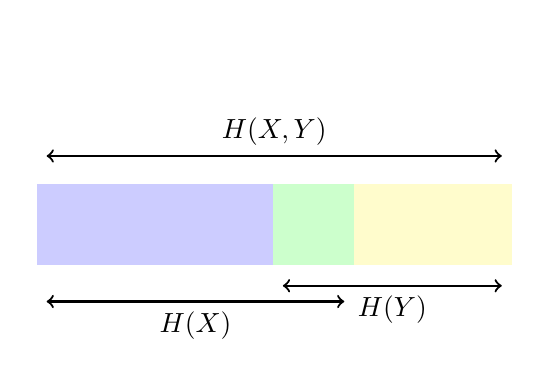
\begin{tikzpicture}
    \draw[help lines,draw=black!0] (0,0) grid (6,4);
    \node[fit={(4,1) (6,2)}, inner sep=0pt, draw=yellow!20, fill=yellow!20,thick] (Y) {};
    \node[fit={(0,1) (3,2)}, inner sep=0pt, draw=blue!20, fill=blue!20,thick] (X) {};
    \node[fit={(3,1) (4,2)}, inner sep=0pt, draw=green!20, fill=green!20,thick] (XcapY) {};
    \node[above = 0.75cm of X.west](Xleft){};
    \node[above = 0.75cm of XcapY.east](Xright){};
    \node[above = 0.75cm of XcapY.west](Yleft){};
    \node[above = 0.75cm of Y.east](Yright){};
    \draw[<->, thick, draw=black] (Xleft) -- (Yright) node[above,midway](HXY){$H(X,Y)$};
    \node[below = 0.85cm of X.west](Xleftb){};
    \node[below = 0.85cm of XcapY.east](Xrightb){};
    \node[below = 0.65cm of XcapY.west](Yleftb){};
    \node[below = 0.65cm of Y.east](Yrightb){};
    \draw[<->, thick, draw=black] (Yleftb) -- (Yrightb) node[below,midway](HY){$H(Y)$};
    \draw[<->, thick, draw=black] (Xleftb) -- (Xrightb) node[below,midway](HX){$H(X)$};
  \end{tikzpicture}

  \end{center}
  
 \end{frame}


\begin{frame}{$H(X,Y)=H(X)+H(Y|X)$}
\begin{center}
  
  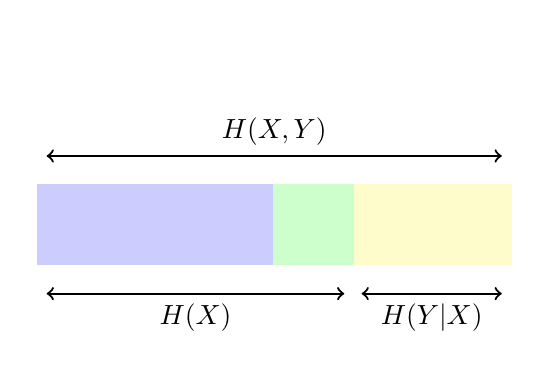
\begin{tikzpicture}
    \draw[help lines,draw=black!0] (0,0) grid (6,4);
    \node[fit={(4,1) (6,2)}, inner sep=0pt, draw=yellow!20, fill=yellow!20,thick] (Y) {};
    \node[fit={(0,1) (3,2)}, inner sep=0pt, draw=blue!20, fill=blue!20,thick] (X) {};
    \node[fit={(3,1) (4,2)}, inner sep=0pt, draw=green!20, fill=green!20,thick] (XcapY) {};
    \node[above = 0.75cm of X.west](Xleft){};
    \node[above = 0.75cm of XcapY.east](Xright){};
    \node[above = 0.75cm of XcapY.west](Yleft){};
    \node[above = 0.75cm of Y.east](Yright){};
    \draw[<->, thick, draw=black] (Xleft) -- (Yright) node[above,midway](HXY){$H(X,Y)$};
    \node[below = 0.75cm of X.west](Xleftb){};
    \node[below = 0.75cm of XcapY.east](Xrightb){};
    \node[below = 0.75cm of Y.west](Yleftb){};
    \node[below = 0.75cm of Y.east](Yrightb){};
    \draw[<->, thick, draw=black] (Yleftb) -- (Yrightb) node[below,midway](HYgX){$H(Y|X)$};
    \draw[<->, thick, draw=black] (Xleftb) -- (Xrightb) node[below,midway](HX){$H(X)$};
  \end{tikzpicture}

  \end{center}
  
 \end{frame}


\begin{frame}{$H(X,Y)=H(Y)+H(X|Y)$}
\begin{center}
  
  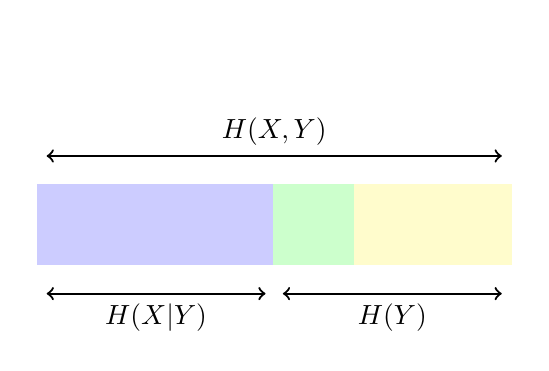
\begin{tikzpicture}
    \draw[help lines,draw=black!0] (0,0) grid (6,4);
    \node[fit={(4,1) (6,2)}, inner sep=0pt, draw=yellow!20, fill=yellow!20,thick] (Y) {};
    \node[fit={(0,1) (3,2)}, inner sep=0pt, draw=blue!20, fill=blue!20,thick] (X) {};
    \node[fit={(3,1) (4,2)}, inner sep=0pt, draw=green!20, fill=green!20,thick] (XcapY) {};
    \node[above = 0.75cm of X.west](Xleft){};
    \node[above = 0.75cm of XcapY.east](Xright){};
    \node[above = 0.75cm of XcapY.west](Yleft){};
    \node[above = 0.75cm of Y.east](Yright){};
    \draw[<->, thick, draw=black] (Xleft) -- (Yright) node[above,midway](HXY){$H(X,Y)$};
    \node[below = 0.75cm of X.west](Xleftb){};
    \node[below = 0.75cm of X.east](Xrightb){};
    \node[below = 0.75cm of XcapY.west](Yleftb){};
    \node[below = 0.75cm of Y.east](Yrightb){};
    \draw[<->, thick, draw=black] (Yleftb) -- (Yrightb) node[below,midway](HYgX){$H(Y)$};
    \draw[<->, thick, draw=black] (Xleftb) -- (Xrightb) node[below,midway](HXgY){$H(X|Y)$};
  \end{tikzpicture}

  \end{center}
  
 \end{frame}


\begin{frame}{Mutual information}
\begin{center}
  
  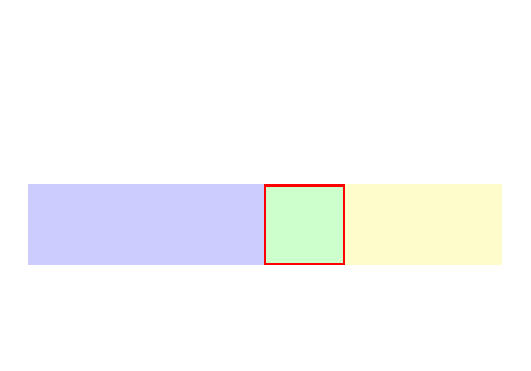
\begin{tikzpicture}
    \draw[help lines,draw=black!0] (0,0) grid (6,4);
    \node[fit={(4,1) (6,2)}, inner sep=0pt, draw=yellow!20, fill=yellow!20,thick] (Y) {};
    \node[fit={(0,1) (3,2)}, inner sep=0pt, draw=blue!20, fill=blue!20,thick] (X) {};
    \node[fit={(3,1) (4,2)}, inner sep=0pt, draw=red, fill=green!20,thick] (XcapY) {};
  \end{tikzpicture}

  \end{center}
  
 \end{frame}


\begin{frame}{Mutual information}
\begin{center}
  
  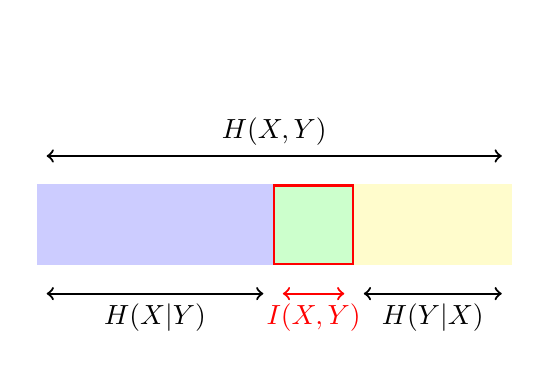
\begin{tikzpicture}
    \draw[help lines,draw=black!0] (0,0) grid (6,4);
    \node[fit={(4,1) (6,2)}, inner sep=0pt, draw=yellow!20, fill=yellow!20,thick] (Y) {};
    \node[fit={(0,1) (3,2)}, inner sep=0pt, draw=blue!20, fill=blue!20,thick] (X) {};
    \node[fit={(3,1) (4,2)}, inner sep=0pt, draw=red, fill=green!20,thick] (XcapY) {};
    \node[above = 0.75cm of X.west](Xleft){};
    \node[above = 0.75cm of XcapY.east](Xright){};
    \node[above = 0.75cm of XcapY.west](Yleft){};
    \node[above = 0.75cm of Y.east](Yright){};
    \draw[<->, thick, draw=black] (Xleft) -- (Yright) node[above,midway](HXY){$H(X,Y)$};
    \node[below = 0.75cm of X.west](Xleftb){};
    \node[below = 0.75cm of XcapY.west](Xrightb){};
    \node[below = 0.75cm of XcapY.east](Yleftb){};
    \node[below = 0.75cm of Y.east](Yrightb){};
    \draw[<->, thick, draw=black] (Yleftb) -- (Yrightb) node[below,midway](HYgX){$H(Y|X)$};
    \draw[<->, thick, draw=black] (Xleftb) -- (Xrightb) node[below,midway](HXgY){$H(X|Y)$};
    \draw[<->, thick, draw=red] (Xrightb) -- (Yleftb) node[below,midway](I){\cred$I(X,Y)$\cbla};
  \end{tikzpicture}

  \end{center}
  
 \end{frame}


\begin{frame}{Mutual information}
\begin{center}
  
  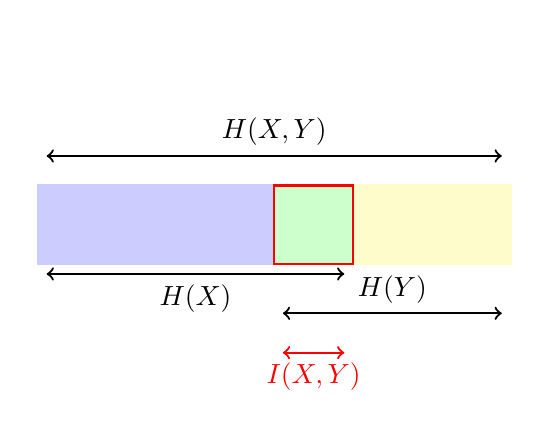
\begin{tikzpicture}
    \draw[help lines,draw=black!0] (0,0) grid (6,4);
    \node[fit={(4,1) (6,2)}, inner sep=0pt, draw=yellow!20, fill=yellow!20,thick] (Y) {};
    \node[fit={(0,1) (3,2)}, inner sep=0pt, draw=blue!20, fill=blue!20,thick] (X) {};
    \node[fit={(3,1) (4,2)}, inner sep=0pt, draw=red, fill=green!20,thick] (XcapY) {};
    \node[above = 0.75cm of X.west](Xleft){};
    \node[above = 0.75cm of XcapY.east](Xright){};
    \node[above = 0.75cm of XcapY.west](Yleft){};
    \node[above = 0.75cm of Y.east](Yright){};
    \draw[<->, thick, draw=black] (Xleft) -- (Yright) node[above,midway](HXY){$H(X,Y)$};
    \node[below = 0.50cm of X.west](Xleftb){};
    \node[below = 1.00cm of XcapY.west](Xrightb){};
    \node[below = 1.50cm of XcapY.west](Xrightbb){};
    \node[below = 0.50cm of XcapY.east](Yleftb){};
    \node[below = 1.50cm of XcapY.east](Yleftbb){};
    \node[below = 1.00cm of Y.east](Yrightb){};
    \draw[<->, thick, draw=black] (Xrightb) -- (Yrightb) node[above,midway](HY){$H(Y)$};
    \draw[<->, thick, draw=black] (Xleftb) -- (Yleftb) node[below,midway](HX){$H(X)$};
    \draw[<->, thick, draw=red] (Xrightbb) -- (Yleftbb) node[below,midway](I){\cred$I(X,Y)$\cbla};
  \end{tikzpicture}

  \end{center}
  
 \end{frame}


\begin{frame}{Mutual information}
\begin{center}
  
  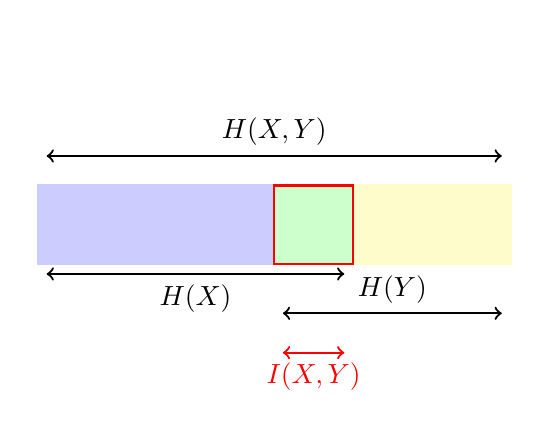
\begin{tikzpicture}
    \draw[help lines,draw=black!0] (0,0) grid (6,4);
    \node[fit={(4,1) (6,2)}, inner sep=0pt, draw=yellow!20, fill=yellow!20,thick] (Y) {};
    \node[fit={(0,1) (3,2)}, inner sep=0pt, draw=blue!20, fill=blue!20,thick] (X) {};
    \node[fit={(3,1) (4,2)}, inner sep=0pt, draw=red, fill=green!20,thick] (XcapY) {};
    \node[above = 0.75cm of X.west](Xleft){};
    \node[above = 0.75cm of XcapY.east](Xright){};
    \node[above = 0.75cm of XcapY.west](Yleft){};
    \node[above = 0.75cm of Y.east](Yright){};
    \draw[<->, thick, draw=black] (Xleft) -- (Yright) node[above,midway](HXY){$H(X,Y)$};
    \node[below = 0.50cm of X.west](Xleftb){};
    \node[below = 1.00cm of XcapY.west](Xrightb){};
    \node[below = 1.50cm of XcapY.west](Xrightbb){};
    \node[below = 0.50cm of XcapY.east](Yleftb){};
    \node[below = 1.50cm of XcapY.east](Yleftbb){};
    \node[below = 1.00cm of Y.east](Yrightb){};
    \draw[<->, thick, draw=black] (Xrightb) -- (Yrightb) node[above,midway](HY){$H(Y)$};
    \draw[<->, thick, draw=black] (Xleftb) -- (Yleftb) node[below,midway](HX){$H(X)$};
    \draw[<->, thick, draw=red] (Xrightbb) -- (Yleftbb) node[below,midway](I){\cred$I(X,Y)$\cbla};
  \end{tikzpicture}

  \end{center}

\crish
$$
I(X,Y)=H(X)+H(Y)-H(X,Y)
$$
\cbla

 \end{frame}


\begin{frame}{Mutual information}
\begin{center}
  
  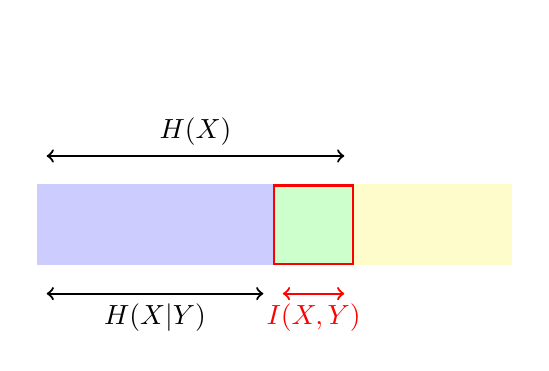
\begin{tikzpicture}
    \draw[help lines,draw=black!0] (0,0) grid (6,4);
    \node[fit={(4,1) (6,2)}, inner sep=0pt, draw=yellow!20, fill=yellow!20,thick] (Y) {};
    \node[fit={(0,1) (3,2)}, inner sep=0pt, draw=blue!20, fill=blue!20,thick] (X) {};
    \node[fit={(3,1) (4,2)}, inner sep=0pt, draw=red, fill=green!20,thick] (XcapY) {};
    \node[above = 0.75cm of X.west](Xleft){};
    \node[above = 0.75cm of XcapY.east](Xright){};
    \node[above = 0.75cm of XcapY.west](Yleft){};
    \node[above = 0.75cm of Y.east](Yright){};
    \draw[<->, thick, draw=black] (Xleft) -- (Xright) node[above,midway](HXY){$H(X)$};
    \node[below = 0.75cm of X.west](Xleftb){};
    \node[below = 0.75cm of XcapY.west](Xrightb){};
    \node[below = 0.75cm of XcapY.east](Yleftb){};
    \node[below = 0.75cm of Y.east](Yrightb){};
    \draw[<->, thick, draw=black] (Xleftb) -- (Xrightb) node[below,midway](HX){$H(X|Y)$};
    \draw[<->, thick, draw=red] (Xrightb) -- (Yleftb) node[below,midway](I){\cred$I(X,Y)$\cbla};
  \end{tikzpicture}

  \end{center}

\crish
$$
I(X,Y)=H(X)+H(Y)-H(X,Y)
$$
\cbla

then substitute \sm{} H(X,Y)=H(Y)+H(X|Y)\fm{} to get

\cred
$$
I(X,Y)=H(X)-H(X|Y)
$$
\cbla

 \end{frame}


\begin{frame}{Mutual information}
\begin{center}
  
  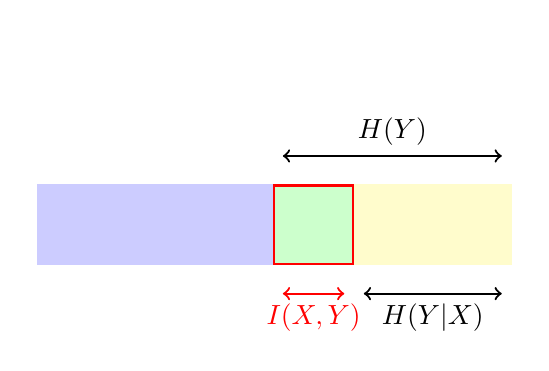
\begin{tikzpicture}
    \draw[help lines,draw=black!0] (0,0) grid (6,4);
    \node[fit={(4,1) (6,2)}, inner sep=0pt, draw=yellow!20, fill=yellow!20,thick] (Y) {};
    \node[fit={(0,1) (3,2)}, inner sep=0pt, draw=blue!20, fill=blue!20,thick] (X) {};
    \node[fit={(3,1) (4,2)}, inner sep=0pt, draw=red, fill=green!20,thick] (XcapY) {};
    \node[above = 0.75cm of X.west](Xleft){};
    \node[above = 0.75cm of XcapY.east](Xright){};
    \node[above = 0.75cm of XcapY.west](Yleft){};
    \node[above = 0.75cm of Y.east](Yright){};
    \draw[<->, thick, draw=black] (Yleft) -- (Yright) node[above,midway](HY){$H(Y)$};
    \node[below = 0.75cm of X.west](Xleftb){};
    \node[below = 0.75cm of XcapY.west](Xrightb){};
    \node[below = 0.75cm of XcapY.east](Yleftb){};
    \node[below = 0.75cm of Y.east](Yrightb){};
    \draw[<->, thick, draw=black] (Yleftb) -- (Yrightb) node[below,midway](HX){$H(Y|X)$};
    \draw[<->, thick, draw=red] (Xrightb) -- (Yleftb) node[below,midway](I){\cred$I(X,Y)$\cbla};
  \end{tikzpicture}

  \end{center}

\crish
$$
I(X,Y)=H(X)+H(Y)-H(X,Y)
$$
\cbla

then substitute \sm{} H(X,Y)=H(Y)+H(X|Y)\fm{} to get

\cred
$$
I(X,Y)=H(Y)-H(Y|X)
$$
\cbla

 \end{frame}

\begin{frame}{All the mutual informations}
\crish
\begin{itemize}
\item $I(X,Y)=H(X)+H(Y)-H(X,Y)$
\item $I(X,Y)=H(X)-H(X|Y)$
\item $I(X,Y)=H(Y)-H(Y|X)$
\item $I(X,Y)=H(X,Y)-H(X|Y)-H(Y|X)$
\end{itemize}
\cbla
\end{frame}

\begin{frame}{Mutual information - direct formula}
  By substituting the formulas for \sm{}H(X)\fm{}, \sm{}H(Y)\fm{} and \sm{}H(X,Y)\fm{} we get
  \crish
  $$
  I(X,Y)=\sum_{i,j} p_{X,Y}(x_i,y_j)\log_2{\frac{p_{X,Y}(x_i,y_j)}{p_X(x_j)p_Y(y_j)}}
  $$
  \cbla
\end{frame}


\begin{frame}{Example}

\begin{center}
\color{purple}
    \begin{tabular}{c|cc}
&$x_0$&$x_1$\\
\hline
$y_0$&$1/4$&$1/4$\\
$y_1$&$1/2$&$0$
    \end{tabular}
    \color{black}
\end{center}
has \sm{}H(X,Y)=3/2\fm{}, \sm{}H(X)\approx 0.81\fm{} and \sm{}H(Y)=1\fm{} so
\crish
$$
I(X,Y)\approx 0.31
$$
\cbla
\end{frame}


\begin{frame}{Mutual information - independent variables}
  \crish
  $$
  I(X,Y)=\sum_{i,j} p_{X,Y}(x_i,y_j)\log_2{\cblu\frac{p_{X,Y}(x_i,y_j)}{p_X(x_j)p_Y(y_j)}}
  $$
  \cbla
  but if \sm{}X\fm{} and \sm{}Y\fm{} are independent \cblu $p_{X,Y}(x_i,y_j)=p_X(x_j)p_Y(y_j)$\cbla{} and hence
    \crish
  $$
  I(X,Y)=0
  $$
  \cbla
\end{frame}


\begin{frame}{Mutual information - independent variables}
  In fact
  \crish
  $$
  I(X,Y)\ge 0
  $$
  \cbla
with equality if and if \sm{}X\fm{} and \sm{}Y\fm{} are independent.
\end{frame}


\begin{frame}{Mutual information - independent variables}
  In fact
    \crish
  $$
  I(X,Y)\ge 0
  $$
  \cbla
  with equality if and if \sm{}X\fm{} and \sm{}Y\fm{} are independent; note that this is equivalent to
    \crish
  $$
  H(X)\ge H(X|Y)
  $$
  \cbla
  with equality if and if \sm{}X\fm{} and \sm{}Y\fm{} are independent; as claimed earlier.
\end{frame}

\begin{frame}{Correlation}
  \crish
  $$
C(X,Y)=\frac{\langle (X-\mu_X)(Y-\mu_Y)\rangle}{\sigma_X\sigma_Y}
$$
\cbla
where \sm{}\mu_X\fm{} is the average of \sm{}X\fm{} and \sm{}\sigma_X\fm{} is its standard deviation with similar notation for \sm{}Y\fm{}.
\end{frame}

\begin{frame}{Correlation}
Consider
\begin{center}
\color{purple}
\begin{tabular}{c|ccc}
&$-1$&$0$&$1$\\
\hline
$1$&$1/4$&$0$  &$1/4$\\
$0$&$0$  &$1/2$&$0$
    \end{tabular}
    \color{black}
\end{center}
then
\crish
$$
C(X,Y)=0
$$
\cbla
whereas \cblu$I(X,Y)=1$\cbla.
\end{frame}

\end{document}

